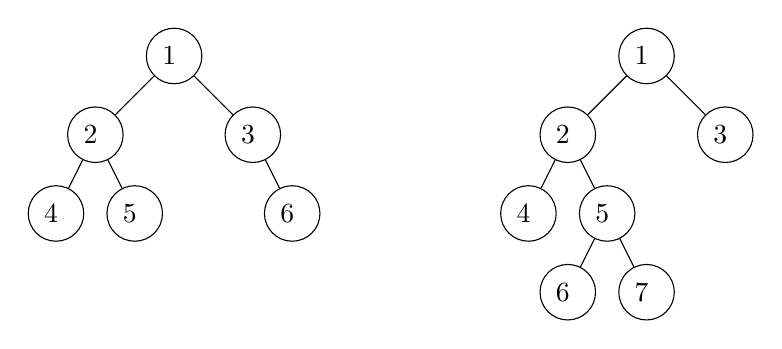
\begin{tikzpicture}[level distance=10mm]
  \tikzstyle{every node}=[circle,draw,text width=0.3cm]
  \tikzstyle{level 1}=[sibling distance=2cm]
  \tikzstyle{level 2}=[sibling distance=1cm]
  \tikzstyle{level 3}=[sibling distance=1cm]
  \node at (2,0) {1}
     child {node {2}
       child {node {4}}
       child {node {5}}
     }
     child {node {3}
       child[fill=none] {edge from parent[draw=none]}
       child {node {6}}
     };

   \node at (8,0) {1}
     child {node {2}
       child {node {4}}
       child {node {5}
         child {node {6}}
         child {node {7}}
      }
     }
     child {node {3}};
\end{tikzpicture}
